\documentclass{article}
\usepackage{amsmath}
\usepackage{amssymb}
\usepackage{graphicx}
\usepackage{xcolor}
\usepackage{tikz}
\begin{document}

\section{Trigonometric Ratios for Special Angles}

\subsection{Special Angles}
In trigonometry, certain angles have special significance due to their simplicity and exact values. The primary special angles are 0°, 30°, 45°, 60°, and 90°.

\subsubsection*{0°}
\begin{minipage}{0.5\textwidth}
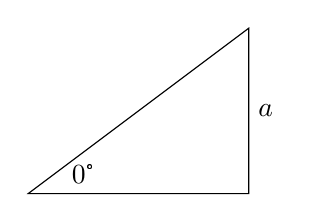
\begin{tikzpicture}[scale=0.7]
    \draw (0,0) -- (4,0) -- (4,3) -- cycle;
    \node[above] at (1,0) {0\textdegree};
    \node[right] at (4,1.5) {$a$};
\end{tikzpicture}
\end{minipage}%
\begin{minipage}{0.5\textwidth}
\[
\begin{aligned}
\sin(0^\circ) &= 0, \\
\cos(0^\circ) &= 1, \\
\tan(0^\circ) &= 0.
\end{aligned}
\]
\end{minipage}

\subsubsection*{30°}
\begin{minipage}{0.5\textwidth}
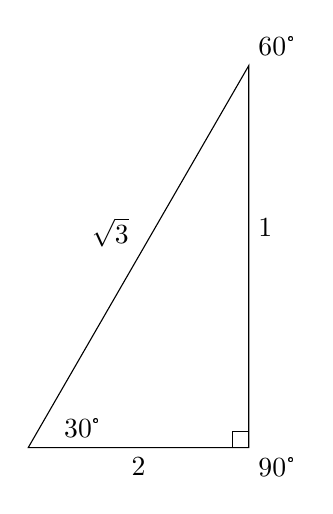
\begin{tikzpicture}[scale=0.7]
    \draw (0,0) -- (4,0) -- (4,{4*sqrt(3)}) -- cycle;
    \draw (3.7,0) -- (3.7,0.3) -- (4,0.3);
    \node[above left] at (1.5,0) {30\textdegree};
    \node[above right] at (4,{4*sqrt(3)}) {60\textdegree};
    \node[below right] at (4,0) {90\textdegree};
    \node[right] at (4,4) {$1$};
    \node[below] at (2,0) {$2$};
    \node[above left] at (2,{2*sqrt(3)}) {$\sqrt{3}$};
\end{tikzpicture}
\end{minipage}%
\begin{minipage}{0.5\textwidth}
\[
\begin{aligned}
\sin(30^\circ) &= \dfrac{1}{2}, \\
\cos(30^\circ) &= \dfrac{\sqrt{3}}{2}, \\
\tan(30^\circ) &= \dfrac{1}{\sqrt{3}}.
\end{aligned}
\]
\end{minipage}

\subsubsection*{45°}
\begin{minipage}{0.5\textwidth}
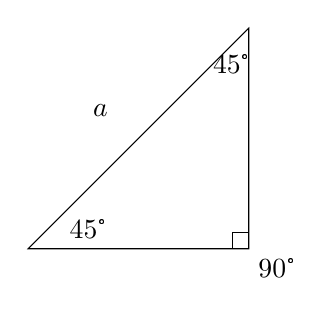
\begin{tikzpicture}[scale=0.7]
    \draw (0,0) -- (4,0) -- (4,4) -- cycle;
    \draw (3.7,0) -- (3.7,0.3) -- (4,0.3);
    \node[below left] at (1.6,0.7) {45\textdegree};
    \node[above left] at (4.2,3) {45\textdegree};
    \node[below right] at (4,0) {90\textdegree};
    \node[right] at (1,2.5) {$a$};
\end{tikzpicture}
\end{minipage}%
\begin{minipage}{0.5\textwidth}
\[
\begin{aligned}
\sin(45^\circ) &= \dfrac{\sqrt{2}}{2}, \\
\cos(45^\circ) &= \dfrac{\sqrt{2}}{2}, \\
\tan(45^\circ) &= 1.
\end{aligned}
\]
\end{minipage}

\subsubsection*{60°}
\begin{minipage}{0.5\textwidth}
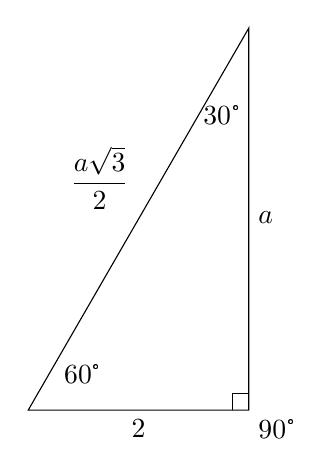
\begin{tikzpicture}[scale=0.7]
    \draw (0,0) -- (4,0) -- (4,{4*sqrt(3)}) -- cycle;
    \draw (3.7,0) -- (3.7,0.3) -- (4,0.3);
    \node[below left] at (1.5,1) {60\textdegree};
    \node[above right] at (3,5) {30\textdegree};
    \node[below right] at (4,0) {90\textdegree};
    \node[right] at (4,3.5) {$a$};
    \node[below] at (2,0) {$2$};
    \node[above left] at (2,{2*sqrt(3)}) {$\dfrac{a\sqrt{3}}{2}$};
\end{tikzpicture}
\end{minipage}%
\begin{minipage}{0.5\textwidth}
\[
\begin{aligned}
\sin(60^\circ) &= \dfrac{\sqrt{3}}{2}, \\
\cos(60^\circ) &= \dfrac{1}{2}, \\
\tan(60^\circ) &= \sqrt{3}.
\end{aligned}
\]
\end{minipage}

\subsubsection*{90°}
\begin{minipage}{0.5\textwidth}
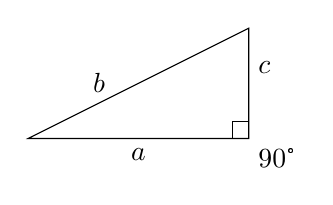
\begin{tikzpicture}[scale=0.7]
    \draw (0,0) -- (4,0) -- (4,2) -- cycle;
    \draw (3.7,0) -- (3.7,0.3) -- (4,0.3);
    \node[below right] at (4,0) {90\textdegree};
    \node[right] at (1,1) {$b$};
    \node[below] at (2,0) {$a$};
    \node[above right] at (4,1) {$c$};
\end{tikzpicture}
\end{minipage}%
\begin{minipage}{0.5\textwidth}
\[
\begin{aligned}
\sin(90^\circ) &= 1, \\
\cos(90^\circ) &= 0 , \\
\tan(90^\circ) &= \text{undefined}.
\end{aligned}
\]
\end{minipage}

\end{document}
